
%\chapter{Introdução}


\chapter{Introdução}

Estamos vivendo um momento em nossa sociedade onde somos bombardeados por campanhas de marketing que nos convencem que precisamos de determinado produto ou serviço. Para produtos destinados ao público infantil, temos um agravante, pois as crianças possuem pouco ou nenhum conhecimento sobre como funciona o dinheiro, neste ambiente, a educação financeira torna-se imprescindível desde as idades iniciais.   Desta forma, tendo dimensão da importância do assunto, foi instaurada, por meio do decreto 7.397/2010, a Estratégia Nacional da Educação Financeira - ENEF.
\begin{citacao}
	Fica instituída a Estratégia Nacional de Educação Financeira - ENEF com a finalidade de promover a educação financeira e previdenciária e contribuir para o fortalecimento da cidadania, a eficiência e solidez do sistema financeiro nacional e a tomada de decisões conscientes por parte dos consumidores.
	\cite{decreto_7397}
\end{citacao} 











-------------------------------------------------------------------------------------------------------------------------

A introdução apresenta os objetivos do trabalho, bem como as razões de sua elaboração. Tem caráter didático de apresentação.

Deve abordar:
\begin{enumerate}[noitemsep,nosep,labelindent=\parindent,leftmargin=*,label={\alph*}) ] 
	\item o problema de pesquisa, proposto de forma clara e objetiva;
	\item os objetivos, delimitando o que se pretende fazer;
	\item a justificativa, destacando a importância do estudo;
	\item apresentar as definições e conceitos necessários para a compreensão do estudo;
	\item apresentar a forma como está estruturado o trabalho e o que contém cada uma de suas partes.
\end{enumerate}

O desenvolvimento é a demonstração lógica de todo o trabalho, detalha a pesquisa ou o estudo realizado. Explica, discute e demonstra a pertinência das teorias utilizadas na exposição e resolução do problema. 

O desenvolvimento pode ser subdivido em seções e subseções com nomenclaturas definidas pelo autor conforme conteúdo apresentado. 

Regras de apresentação da Capa




\begin{table}[!htbp]
	\centering
%	\small
	\renewcommand{\arraystretch}{1.3}
	\caption{Formatação do papel e fonte.}%
	\label{tab:quadro_exemplo}
	\begin{tabular}{| L{3cm} | L{11cm} | }
		\hline
		\textbf{Elementos}		& \textbf{Apresentação gráfica}	 		\\ 
		\hline
		\hline
%		& \multicolumn{2}{c}{\textbf{Dispositivos}} \\
%		\cmidrule(lr{0.5ex}){2-3}
		\multirow{2}{*}[-12pt]{\textbf{Papel}}	& Branco, em formato A4 (21 cm x 29,7 cm)
													Os textos devem ser digitados na cor preta, podendo-se utilizar outras cores somente para as ilustrações (não são considerados o título, a fonte e legenda da ilustração, que devem ser na cor preta)
													Os textos devem ser digitados no anverso da folha (frente), pois os trabalhos estarão disponíveis somente em formato digital 
													 \\ 
													 \cline{2-2}
												& 	 Os elementos pré-textuais (folha de rosto, agradecimentos, resumo etc.), textuais (seções primárias) e pós-textuais (referências, apêndice etc.) devem iniciar sempre em nova página 
												\\
		\hline
		\hline
		\textbf{Margens} 			& Esquerda e superior: 3,0 cm \newline
									Direita e inferior: 2,0 cm	\\
		\hline
		\hline
		 				& Arial ou Times New Roman (padronizar uma fonte para todo o trabalho).  \\ \cline{2-2}
		\textbf{Fonte}	& Tamanho 12 para todo o trabalho 	\\ \cline{2-2}
						& Tamanho 10: citações com mais de três linhas, paginação, notas de rodapé, dados internacionais de catalogação na publicação, legendas e fontes das ilustrações e tabelas \\ 
		\hline
	\end{tabular}
	\vspace{2mm}
	\fonte{Elaborado pelos autores (2020), com base na NBR 14724 (2011).}
\end{table}


\section{SEÇÃO SECUNDÁRIA}

A ABNT indica a elaboração de uma lista de ilustrações com todos os itens arrolados e designados por seu nome específico, conforme a ordem que aparecem no texto (Figura 1, Fotografia 1, Gráfico 1, Quadro 1, entre outros). Também recomenda, quando necessário, a elaboração de lista própria para cada tipo de ilustração. No entanto, não determina um número mínimo de ilustrações para tal lista específica.

Nesse caso, a BU Udesc estabelece a elaboração de listas específicas para cada tipo de ilustração somente quando existirem muitos itens de cada tipo: cinco (5) ou mais (mais do que cinco desenhos, gráficos etc.). Caso contrário, elabora-se uma única lista, denominada “Lista de ilustrações” com os elementos ordenados conforme aparecem no texto, nominando-os “Figura” e, portanto, não diferenciando fotografia, gráfico, quadro e outros.


\subsection{Seção terciária}

O vídeo fornece uma maneira poderosa de ajudá-lo a provar seu argumento. Ao clicar em Vídeo Online, você pode colar o código de inserção do vídeo que deseja adicionar.

\subsubsection{Seção quaternária}

O vídeo fornece uma maneira poderosa de ajudá-lo a provar seu argumento. Ao clicar em Vídeo Online, você pode colar o código de inserção do vídeo que deseja adicionar. Você também pode digitar uma palavra-chave para pesquisar online o vídeo mais adequado ao seu documento. 


\begin{figure}
	\centering
	\caption{Exemplo de paginação.}
	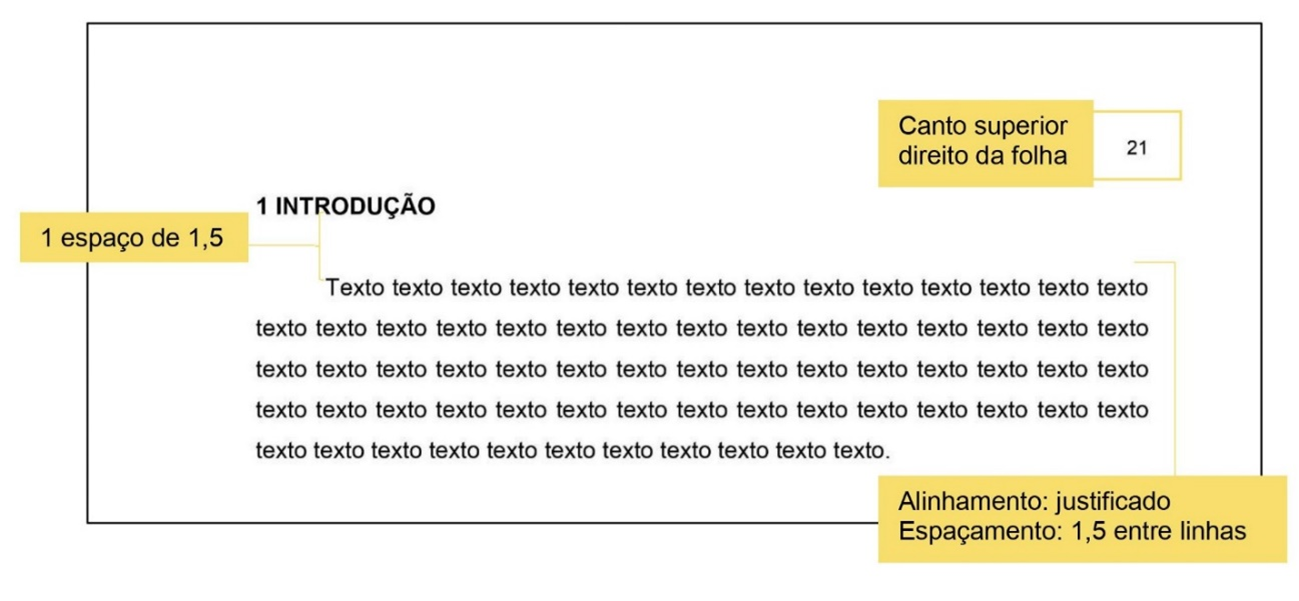
\includegraphics[scale=1]{Textuais/Picture1.png}
	\fonte{Elaborada pelos autores (2020), com base na NBR 14724 (2011).}
\end{figure}


\subsubsubsection{Seção quinaria}



O vídeo fornece uma maneira poderosa de ajudá-lo a provar seu argumento. Ao clicar em Vídeo Online, você pode colar o código de inserção do vídeo que deseja adicionar. Você também pode digitar uma palavra-chave para pesquisar online o vídeo mais adequado ao seu documento. Para dar ao documento uma aparência profissional, o Word\footnote{O Microsoft Word é um processador de texto produzido pela Microsoft Office foi criado por Richard Brodie para computadores IBM PC com o sistema operacional DOS em 1983.} fornece designs de cabeçalho, rodapé, folha de rosto e caixa de texto que se complementam entre si. Por exemplo, você pode adicionar uma folha de rosto, um cabeçalho e uma barra lateral correspondentes.

\begin{table}[!htbp]
	\centering
	%	\small
	\renewcommand{\arraystretch}{1.1}
	\caption{Modelo de tabela.}%
	\label{tab:tabela_exemplo}
	\begin{tabular}{ L{4cm}  R{3cm} || L{4cm}  R{3cm}  }
		\hline
		Município		& População Estimada & Município		& População Estimada 		\\ 
		\hline
		Abdon Batista		& 2630	& Bom Jesus				& 2821 \\ 
		Abelardo Luz		& 17717	& Bom Jesus do Oeste	& 2156 \\ 
		Agrolândia			& 10272	& Bom Retiro			& 9598 \\ 
		Agronômica			& 5306	& Bombinhas				& 17477 \\ 
		Água Doce			& 7132	& Botuverá				& 4943 \\ 
		Águas de Chapecó	& 6379	& Braço do Norte		& 31765 \\ 
		\hline
	\end{tabular}
	\vspace{2mm}
	\fonte{Adaptado de IBGE (2015).}
\end{table}

Clique em Inserir e escolha os elementos desejados nas diferentes galerias.

\begin{figure}
	\centering
	\caption{População.}
	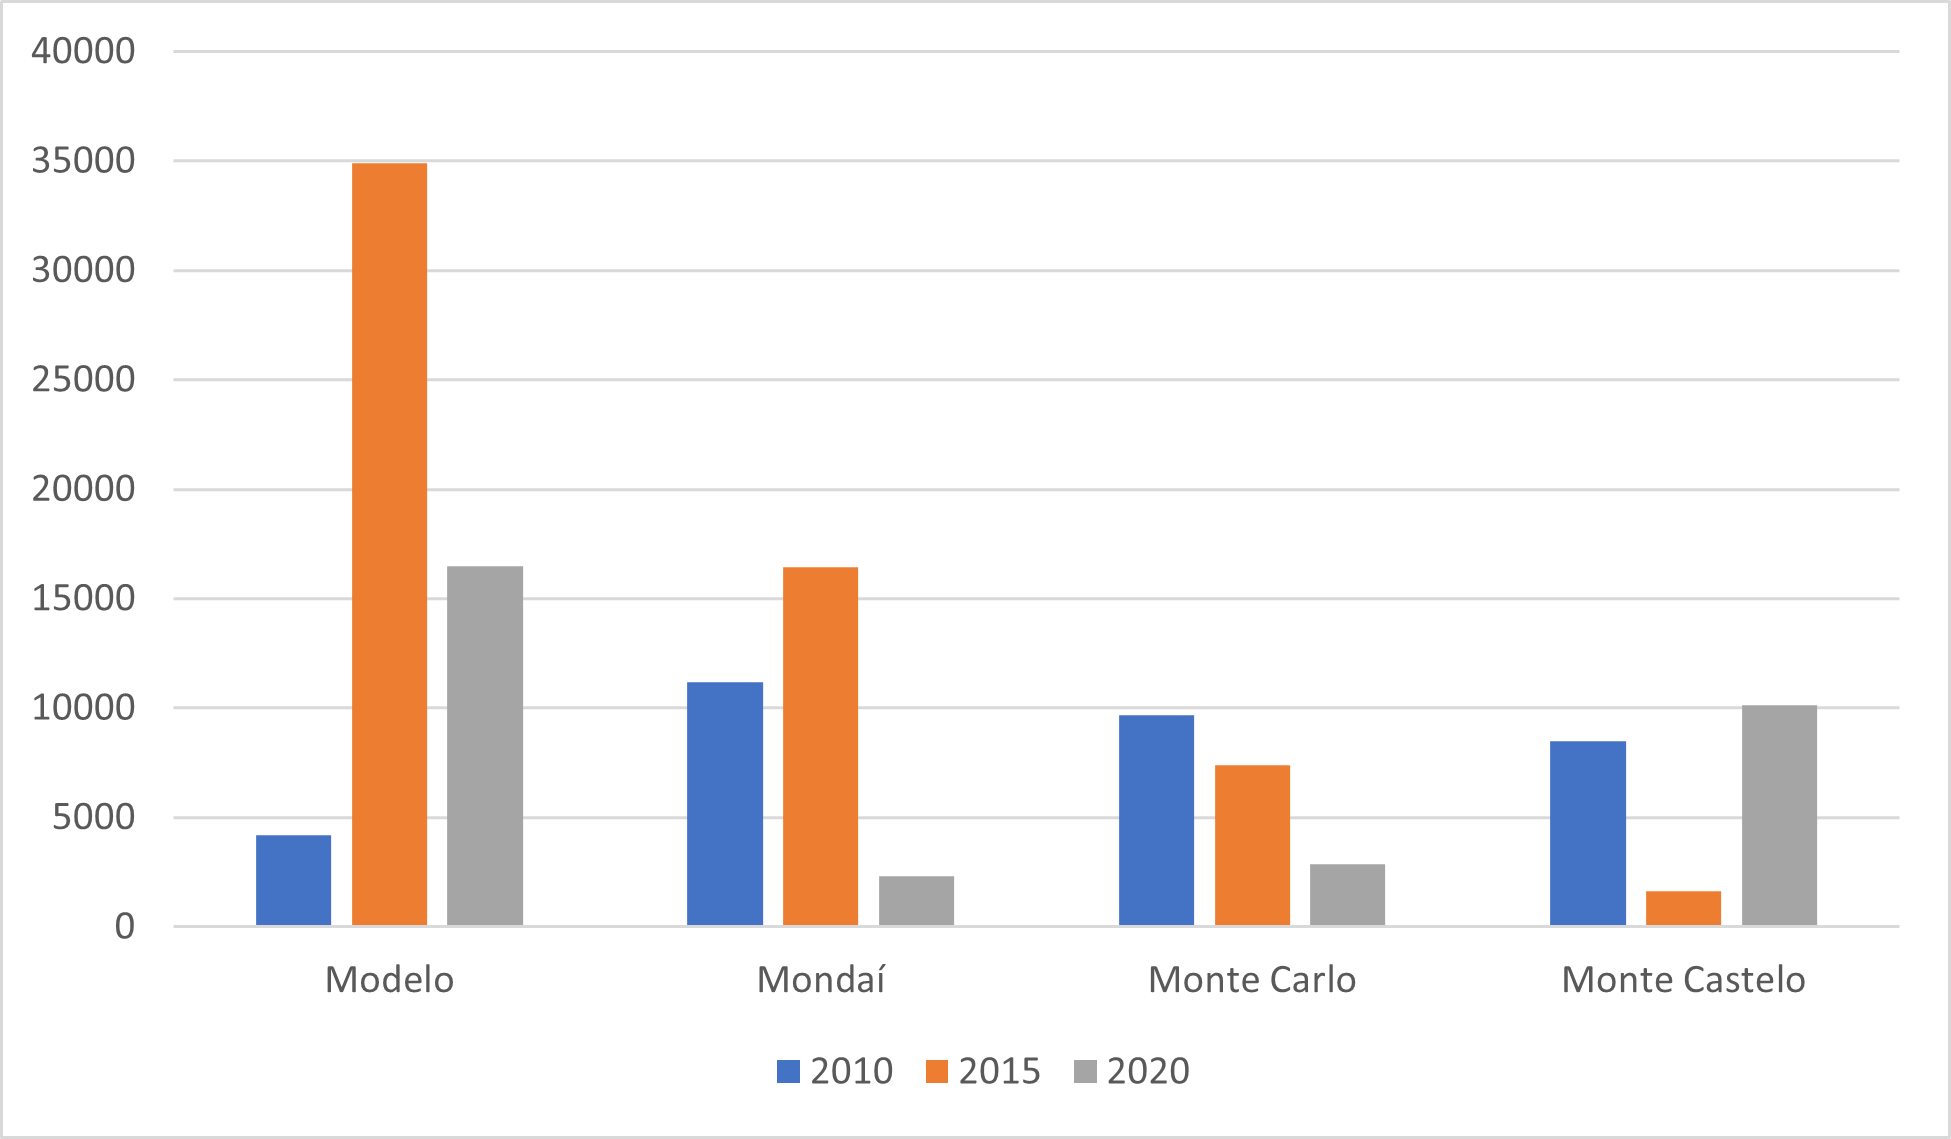
\includegraphics[scale=1]{Textuais/Picture2.png}
	\fonte{\me{2020}}
\end{figure}

As chamadas às equações e fórmulas, no texto, devem ser feitas da seguinte forma: equação (1), fórmula (2).

\textbf{Exemplo 1:}
O Teorema de Pitágoras, é uma equação \eqref{eq:eq1} que pode ser aplicada em qualquer triângulo retângulo (triângulo que tem um ângulo de 90°).
\begin{equation} \label{eq:eq1}
a^2 + b^2 = c^2 
\end{equation}

\textbf{Exemplo 2:}
A dopamina é um composto orgânico de função mista álcool, fenol e amina que apresenta fórmula \eqref{eq:form1} molecular:
\begin{equation} \label{eq:form1}
\ch{C8 + H11NO2} 
\end{equation}

\textbf{Exemplo 3:}
O modelo matemático de Huang (HUG), dado pelas equações \eqref{eq:eq3} e \eqref{eq:eq4}, foi elaborado com o intuito de fornecer uma descrição mais simples do crescimento bacteriano.
\begin{gather} 
	y(t) = y_0 + y_{max} -\ln{[e^{y_0}  + (e^{y_{max}} -e^{y_0} )  e^{-u_{max}\beta(t)} ]}   \label{eq:eq3}  \\
	\beta(t) = t + \frac{1}{4}\ln\left( \frac{1+ e^{-4(t-\lambda)} }{1+ e^{4(\lambda)} }\right) \label{eq:eq4}
\end{gather}
\noindent onde $y(t)$ corresponde ao logaritmo natural da concentração celular (log UFC/g) no instante $t$ (dias), $y_{max}$ é o logaritmo natural da população bacteriana (log UFC/g) final, $y_0$ corresponde ao logaritmo natural da população bacteriana inicial (log UFC/g) e $\beta(t)$ é a função de transição.

\textbf{Exemplo 4:}
Para o cálculo da intensidade fórmula \eqref{eq:eq5} de Intensidade-Duração-Frequência apresentada, os valores encontrados seguindo os parâmetros apresentados e como o resultado é dado em mm/h haverá também a sua conversão para m/s.
\begin{gather} 
	i = \frac{K T^m}{(t+b)^n}   \label{eq:eq5}  \\[2ex]
		i = \frac{\num{625.58} \cdot 5^{\num{0.171}}  }{(60+\num{8.89})^{\num{0.961}}} \\[2ex]
		i = \num{44.222} \cdot \frac{\si{mm}}{\si{h}} \cdot \frac{1\mathrm{m}}{\SI{1000}{mm}} \cdot \frac{\SI{1}{h}}{\SI{3600}{s}} 	
\end{gather}
\noindent onde, $i$ é a intensidade média máxima de precipitação, em mm/h; $T$ é o Período de retorno, em anos; $t$ é a duração da chuva, em minutos; $k,m,b,n$ são os parâmetros da equação determinados para cada local.


As citações diretas com até três linhas ``[...] devem estar contidas entre aspas duplas. As aspas simples são utilizadas para indicar citação no interior da citação.'' (ABNT, 2002, p. 2). Devem apresentar autor, ano e página. Quando a indicação de autor estiver dentro de parênteses, o sobrenome deve ser em letra maiúscula. 


As citações diretas com mais três linhas ``[...] devem ser destacadas com recuo de 4 cm da margem esquerda, com letra menor que a do texto utilizado e sem as aspas.'' (ABNT, 2002, p. 2). Ou seja, utilizar fonte tamanho 10 para as citações diretas longas, com espaçamentos simples entre linhas. As citações devem ser precedidas e antecedidas por um (1) espaço de 1,5 entrelinhas. 


Nas citações indiretas não há necessidade de usar aspas e indicar a página, considerando que é uma paráfrase. Faz-se necessário apresentar o autor e ano.




\noindent Exemplo referência de livro: \cite{exemplo_livro}

\noindent Exemplo referência de livro em meio eletrônico: \cite{exemplo_livroe}

\noindent Exemplo referência de trabalho acadêmico (Dissertação de Mestrado): \cite{exemplo_dissertacao}

\noindent Exemplo referência de trabalho acadêmico (Tese de Doutorado): \cite{exemplo_tese}

\noindent Exemplo referência de artigo: \cite{exemplo_artigo}


\textbf{Para outras referências ver Manual Udesc}: \url{https://www.udesc.br/bu/manuais}








